%=====================================================================
%  VOR: Vector-adaptive Online Reference-reallocation EA
%       for Large-Scale and Constrained Multi-Objective Optimization
%  (Battlefield routing: one codebase services D=10 constrained
%   and D=300 large-scale battlefields)
%
%  Target: Applied Soft Computing (Elsevier Q1) — applied/computational
%          journal track (no theorems required; SOTA comparison +
%          significance tests required).
%  Compile: pdflatex main -> bibtex main -> pdflatex main -> pdflatex main
%           (requires elsarticle.cls in same dir or TEXPATH)
%=====================================================================
\documentclass[preprint,12pt]{elsarticle}

\usepackage{amsmath,amssymb}
\usepackage{booktabs}
\usepackage{array}
\usepackage{graphicx}
\usepackage{algorithm}
\usepackage{algorithmic}
\usepackage{subcaption}
\usepackage{multirow}
\usepackage{ragged2e}
\usepackage{url}
\usepackage[hidelinks]{hyperref}
\usepackage{microtype}
\setlength{\emergencystretch}{2em}
\setlength{\parindent}{0pt}
\usepackage{setspace}
\setstretch{1.12}

\graphicspath{{../results/figs/out/}{../results/figs/pf/}}

% 允许在正文中直接画矢量图（期刊要求 600DPI 矢量）
\usepackage{pdflscape}

\journal{Applied Soft Computing}

\begin{document}

\begin{frontmatter}

\title{\hyphenpenalty=10000\ Battlefield-Adaptive Evolutionary
Algorithm with Online Reference-Reallocation and Quantile
$\varepsilon$-Grid Selection for Large-Scale and Constrained
Multi-Objective Optimization}

\author[a]{Yuxuan Zhang\corref{cor1}}
\ead{3150644070@qq.com}
\cortext[cor1]{Corresponding author.}
\address[a]{Graduate School, Army Engineering University of
PLA, Nanjing, China}

\begin{abstract}
Large-scale multi-objective optimization in which the number of decision
variables $D$ reaches several hundreds remains one of the most challenging
open problems in evolutionary multi-objective optimization. Reference-vector
mechanisms (NSGA-III, RVEA) lose diversity as the non-dominated set must be
distributed across a growing objective space, and classical crossover such as
SBX loses directed-convergence capability as the decision space grows. Most
existing dimension-adaptive algorithms, however, target a \emph{single}
battlefield: large-$D$ (\textsc{LSMOP}, \textsc{DTLZ2}-300D) \emph{or}
constrained low-dimensional (\textsc{CF}, \textsc{MW}), and cannot be applied
to both without re-implementation. This paper proposes
\textbf{VOR} (\emph{Vector-adaptive Online Reference-reallocation EA}), a
dimension-adaptive framework whose central mechanism is a
\emph{battlefield routing} rule: a single codebase services the
large-scale ($D=300$) and the constrained low-dimensional ($D=10$--$60$)
battlefields, with the variation operator, environmental selection and
reference-vector reallocation jointly gated by the initial IGD scale, the
decision dimension, and the presence of constraints.
\textbf{Core contributions:}
(i)~a quantile $\varepsilon$-grid environmental selection (\textsc{Q-EPS})
that keeps the population on the true Pareto front at PPS$\,\approx\,N$ on
irregular fronts where EDD's fixed 10-bin grid collapses to PPS 24--27
(\textsc{CF1}/\textsc{LSMOP6});
(ii)~an online reference-vector reallocation (\textsc{ORA}) that, every 10
generations, clusters the front-1 decision space and pulls NBI reference
vectors toward the cluster principal directions, repairing NSGA-III's
reference/front misalignment on \textsc{MaF14};
(iii)~an IGD-derivative-gated operator switch that, at \emph{any} dimension,
auto-switches APD$\to$DSG$\to$GDV when the IGD derivative stalls for 10
generations; and
(iv)~the \emph{battlefield routing} rule that makes one codebase service
$D\in\{10,30,60,300\}$ without hand-tuned dimension gates.
\textbf{Main results} (6 problems $\times$ 30 seeds, N=100, G=200): on the
five-algorithm set \{NSGA-2, RVEA, MOEA/D, EDD(v12), VOR\}, VOR attains the
first IGD rank on 3 of 6 problems (\textsc{ZDT1}, \textsc{LSMOP1},
\textsc{LSMOP6}), the second on \textsc{DTLZ2}-300D and the third on
\textsc{MaF14}/\textsc{CF1}, with a statistically significant IGD advantage
over \textsc{EDD} on \textsc{ZDT1}, \textsc{LSMOP1} and \textsc{CF1}
(30-seed Wilcoxon, $p<10^{-5}$, rank-biserial effects $0.5$--$1.0$).
\textbf{Honest limitations:} (a)~against the three 2026 state-of-the-art
algorithms \textsc{FDSEA}/\textsc{GDVTSF}/\textsc{MOEA-IB}
($D=300$, 30 seeds, the same seed protocol as the \textsc{VOR} runs),
\textsc{VOR} is \emph{not} the combined IGD/HV winner on the
large-scale battlefield: \textsc{FDSEA} outperforms \textsc{VOR} on all
three $D=300$ instances (\textsc{LSMOP1} $0.143$ vs $0.706$; \textsc{LSMOP6}
$0.668$ vs $1.608$; \textsc{DTLZ2}-300D $0.065$ vs $0.749$); VOR's
differentiating value is the \emph{single-codebase coverage} of the
constrained low-dimensional battlefield where the three SOTA algorithms
have no published $D=10$--$60$ benchmark;
(b)~on \textsc{CF1} (constrained, $D=10$), MOEA/D's decomposition still
retains a structural advantage (IGD $0.010$ vs VOR $0.063$);
(c)~\textsc{MaF14} exhibits the seed-invariance property
(std$=0.0000$) shared by the EDD family. We therefore position VOR as the
\emph{battlefield-broadening} member of the EDD lineage: it fixes part of
the constrained low-dimensional PPS collapse that was the original EDD\_cf's
defining weakness while preserving the large-scale robustness property, and
we report its quantified residual boundary on the $D=300$ battlefield
against the 2026 SOTA in full.
\end{abstract}

\begin{keyword}
large-scale multi-objective optimization \sep
battlefield-adaptive evolutionary algorithm \sep
quantile epsilon-grid selection \sep
online reference-vector reallocation \sep
IGD-gated operator switching \sep
constrained multi-objective optimization
\end{keyword}

\end{frontmatter}

%=====================================================================
\section{Introduction}
\label{sec:intro}

\subsection{The two-battlefield challenge}

Multi-objective optimization (MOO) problems with a large decision dimension
$D$ (hundreds to thousands) arise wherever the number of design variables far
exceeds the number of objectives. Such problems are distinct from classical
many-objective problems (MaOPs, $M\ge 5$): even with only three objectives,
the search space grows as $2^D$, and the interplay between convergence and
diversity is fundamentally different from the low-dimensional regime in which
most existing evolutionary multi-objective optimizers (EMOAs) are tuned.
Classical EMOAs fail on large-scale decision spaces in two ways. First,
reference-vector mechanisms (NSGA-III~\cite{deb2014an}, RVEA~\cite{cheng2016a},
MOEA/D~\cite{qingfuzhang2007moead}) distribute the population across the
objective space using a fixed number of reference points; as $D$ grows the
non-dominated front becomes dense in objective space and a fixed reference
set cannot resolve it, so diversity degrades. Second, scalarized offspring
operators (SBX, polynomial mutation) assume low-dimensional structure in
their crossover distribution; in high-$D$ search spaces they behave as
essentially undirected random walks, and convergence slows by several orders
of magnitude.

A complementary, equally important regime is the
\emph{constrained low-dimensional} battlefield. Benchmark families such
as \textsc{CF1}--\textsc{CF6} ($D=10$, $M=3$) and \textsc{MW1}--\textsc{MW3}
($D=10$--$15$, $M=3$) test constraint handling, while the
\textsc{MaF} family ($D=60$, $M=3$) introduces irregular, non-smooth
Pareto fronts that stress the reference-vector alignment. The
large-scale benchmark families used here ---
\textsc{LSMOP} (LSMOP1--9)~\cite{cheng2017test} and the constrained
\textsc{CF}/\textsc{MW}/\textsc{MaF} suites --- follow the standard
\textsc{PlatEMO}~\cite{chen2014platemo} protocol. Most large-scale
solvers (DSG-EA~\cite{zou2024two},
PH-LSMAEA~\cite{wang2024population},
a fuzzy decision-variable
framework~\cite{yang2023fuzzy},
FDSEA~\cite{fdsea2024},
GDVTSF~\cite{gdvtsf2025},
MOEA-IB~\cite{moeaib2025})
are designed for $D\ge 100$ and either skip the constrained low-dimensional
regime or collapse on it. The \textsc{EDD} lineage (EDD v12) addressed this
by grafting dimension-aware gating: when $D\ge 100$ it uses an
$\varepsilon$-grid environmental selection with directed decision-space
operators, otherwise it falls back to an adaptive-Pareto-distance
(\textsc{APD}) + reference-vector + \textsc{SMS} architecture. However, EDD
retains two documented structural weaknesses: (i) its fixed 10-bin
$\varepsilon$ grid collapses PPS on the irregular \textsc{MaF14} front
(PPS 8--97 across seeds) and stagnates at IGD 0.86 (seed-invariant,
std$=0.0000$); (ii) its fixed 10-bin grid and the convergence-freeze gate
($\mathrm{IGD}<0.02$) prematurely freeze the high-$D$ \textsc{LSMOP6}
front (PPS 24.6) and the constrained \textsc{CF1} (PPS 24.2).

\subsection{The single-codebase gap and our approach}

The gap we target is \emph{not} a single-battlefield SOTA (the 2026 SOTA
algorithms already win on $D=300$ \textsc{LSMOP}/\textsc{DTLZ2}); the gap is
that \emph{no published algorithm services both battlefields from one
codebase} without hand-tuned dimension gates. We propose
\textbf{VOR} (Vector-adaptive Online Reference-reallocation EA), whose
central mechanism is a \emph{battlefield routing} rule that reads the
initial IGD scale, the dimension $D$ and the presence of constraints
\textsc{hasCon}, and routes to one of three operator regimes:
\begin{itemize}
\item \textsc{DSG} (directed-sampling operator) when
$D\ge 100$ \emph{and} $\mathrm{IGD}_0\ge 15$ (large-scale hard-convergence
battlefield: \textsc{LSMOP6}, \textsc{DTLZ2}-300D), or when
$30\le D<100$ \emph{and} \textsc{hasCon} (\textsc{MaF14});
\item \textsc{APD} + \textsc{SMS} (adaptive-Pareto-distance +
  \textsc{SMS-EMO} switch) when $D<100$ and \textsc{hasCon}$=0$
  (\textsc{ZDT1} simple battlefield), and when $D<30$ and \textsc{hasCon}$=1$
  (\textsc{CF1} constrained low-dimensional battlefield);
\item \textsc{GDV} (generational-difference-vector local search) is
injected only as a stagnation-triggered escape when
$\mathrm{stagn}\ge 20$ and the regime is not already \textsc{SMS}/\textsc{GDV}.
\end{itemize}
The routing is computed \emph{once} at the start of the run (after the
initial population is evaluated), so the cost is $O(1)$ per run and the
rest of the code is regime-agnostic. This is the \emph{single-codebase}
property we claim.

\subsection{Contributions}

The main contributions of this paper are:
\begin{enumerate}
\item \textbf{\textsc{Q-EPS}: quantile $\varepsilon$-grid
environmental selection.}
Instead of EDD's fixed 10-bin grid, \textsc{Q-EPS}
re-parses the grid from the 0.25/0.5/0.75/0.9 quantiles
of the \emph{current} non-dominated set every generation, so the
grid tracks the convergence progress.
On \textsc{MaF14}, \textsc{Q-EPS} stabilizes PPS at 100 where
EDD's fixed grid collapses to 8--97 (Section~\ref{sec:qeps}).
\item \textbf{\textsc{ORA}: online reference-vector reallocation.}
Every 10 generations, K-means (cosine distance) clusters the
front-1 decision space into $K=\lceil N/20\rceil$ clusters; the PCA
principal direction $\mathbf{e}_k$ of each cluster pulls the NBI
reference-vector set toward it (learning rate $0.5$), gated by an
IGD-derivative check. This repairs the NSGA-III reference/front
misalignment on irregular \textsc{MaF14} (Section~\ref{sec:ora}).
\item \textbf{IGD-derivative-gated operator switch.} At \emph{any}
dimension, when the IGD relative improvement over 10 generations drops
below $10^{-3}$, VOR auto-switches APD$\to$DSG$\to$GDV and injects
\textsc{CBIM} (convergence-gated boundary immigration) during
$\mathrm{stagn}\in[5,10]$ (Section~\ref{sec:igdgate}).
\item \textbf{Battlefield routing rule (VOR-v2).}
A single $O(1)$-cost routing decision
(initial IGD scale $+~D$ $+$ \textsc{hasCon})
services $D\in\{10,30,60,300\}$ without hand-tuned dimension
gates. This is the differentiating \emph{single-codebase}
property: one framework covers the constrained
low-dimensional \emph{and} the large-scale battlefields
(Section~\ref{sec:routing}).
\end{enumerate}

\subsection{Experiments and honest positioning}

We evaluate VOR on six problems --- \textsc{MaF14} ($M=3$,$D=60$,
constrained, irregular front), \textsc{CF1} ($M=3$,$D=10$, constrained),
\textsc{ZDT1} ($M=2$,$D=30$), \textsc{LSMOP1} ($M=3$,$D=300$),
\textsc{LSMOP6} ($M=3$,$D=300$, initial IGD$\sim 4\times10^4$) and
\textsc{DTLZ2}-300D ($M=3$,$D=300$) --- with 30 independent seeds
(1--30), $N=100$, $G=200$, against four traditional baselines
(\textsc{NSGA-2}, \textsc{RVEA}, \textsc{MOEA/D}, \textsc{EDD} v12) plus
three 2026 SOTA algorithms (\textsc{FDSEA}, \textsc{GDVTSF},
\textsc{MOEA-IB}) on the $D=300$ battlefield. We use a \emph{honest}
positioning:
\begin{itemize}
\item On the \textbf{five-algorithm set} \{\textsc{NSGA-2}, \textsc{RVEA},
  \textsc{MOEA/D}, \textsc{EDD}, \textsc{VOR}\}, VOR attains the first IGD
  rank on 3 of 6 problems (\textsc{ZDT1}, \textsc{LSMOP1}, \textsc{LSMOP6}),
  the second on \textsc{DTLZ2}-300D, and the third on \textsc{MaF14}
  (seed-invariant tie with \textsc{EDD}) and \textsc{CF1}.
\item On the \textbf{three-SOTA set} (\textsc{FDSEA}/\textsc{GDVTSF}/
  \textsc{MOEA-IB}, $D=300$, 30 seeds), \textsc{FDSEA} outperforms VOR on
  all three $D=300$ instances. We therefore \emph{do not claim} that VOR is
  the $D=300$ SOTA; we claim VOR's \emph{differentiating value} is the
  single-codebase coverage of the constrained low-dimensional battlefield
  where the three SOTA algorithms have no published benchmark.
\item \textsc{MaF14} shows the seed-invariance property (std$=0.0000$)
  shared by the EDD family; \textsc{CF1} is a residual boundary where
  MOEA/D's decomposition still retains a structural advantage.
\end{itemize}

\subsection{Paper structure}
Section~\ref{sec:algo} presents the algorithm design.
Section~\ref{sec:exp} reports the experimental protocol, the full IGD/HV
table, the SOTA comparison, and the statistical tests.
Section~\ref{sec:ablation} ablates the battlefield routing.
Section~\ref{sec:disc} discusses the honest boundaries.
Section~\ref{sec:conc} concludes.

%=====================================================================
\section{Algorithm Design}
\label{sec:algo}

\subsection{Notation and problem definition}
\label{sec:notation}
Let $\mathbf{x}=(x_1,\dots,x_D)^\top\in\Omega\subseteq\mathbb{R}^D$ be the
decision vector, $\mathbf{f}:\Omega\to\mathbb{R}^M$ the objective vector,
and $g_j(\mathbf{x})\le 0$, $j=1,\dots,J$ the constraints. We minimize
$\min_{\mathbf{x}\in\Omega}\ \mathbf{f}(\mathbf{x})$ subject to
$g_j(\mathbf{x})\le 0$. The Pareto front (PF) is
$\mathcal{P}^*=\{\mathbf{f}(\mathbf{x}^*)\mid \mathbf{x}^*\ \text{Pareto
optimal}\}$. The Inverted Generational Distance
\begin{equation}
\mathrm{IGD} = \sqrt{\frac{1}{|\mathcal{S}|}\sum_{\mathbf{y}\in\mathcal{S}}
\min_{\mathbf{x}^*\in\mathcal{P}^*}\|\mathbf{y}-\mathbf{x}^*\|^2}
\end{equation}
with $\mathcal{S}$ a 500-point true-front sample (lower is better). The
Hypervolume (HV) uses a reference point $\mathbf{r}=1.1\cdot\max(\mathrm{PF})$
(higher is better). PPS is the number of non-dominated solutions in the final
population; PPS$=N$ is ideal.

\subsection{HCEAV4 architecture base}
\label{sec:base}
VOR inherits the EDD/HCEAV4 three-layer architecture:
\begin{itemize}
\item \textbf{\textsc{APD} (Adaptive Pareto front Distancing):} NBI
  reference vectors $\mathbf{V}$ as anchors; each solution associates with
  its closest reference vector (cosine angle $d_{\min}$, using only the
  first $\min(M,2)$ objective dimensions to avoid the MBI-angle density
  collapse on $M=3$ problems); APD distance
  $d_{\mathrm{APD}}=(1+M\theta d_{\min}/\gamma)\cdot\|\mathbf{f}\|$, with
  $\theta=(g/G)^{\alpha}$ decaying over generations ($\alpha=2$).
\item \textbf{HV-validated switch:} at $g=0.5G,0.6G,0.7G$ VOR probes the
  \textsc{SMS} environmental selection; if the HV improves it permanently
  switches (\textsc{EDD} reaches IGD$=0.004$ on \textsc{ZDT1} precisely via
  a gen-100 \textsc{SMS} switch). The convergence guard disables the switch
  only when $\mathrm{IGD}<0.02$ (the previous $0.1$ guard mis-froze
  \textsc{CF1}).
\item \textbf{Terminal HV polish:} from $g\ge 0.9G$ (constrained problems
  $0.75G$), every $5$ generations (every $4$ for constrained) a small
  perturbation is applied to a random individual and accepted only if it
  does not worsen its parent.
\end{itemize}

\subsection{\textsc{Q-EPS}: quantile $\varepsilon$-grid environmental
selection}
\label{sec:qeps}
\emph{Motivation.} EDD's fixed 10-bin $\varepsilon$ grid collapses PPS on
the irregular \textsc{MaF14} front (PPS 8--97) and on \textsc{CF1}
(PPS 24.2). \textsc{Q-EPS} re-parses the grid from the 0.25/0.5/0.75/0.9
quantiles of the \emph{current} non-dominated objective matrix
$\mathbf{F}$ every generation, so the grid tracks the convergence progress:
\begin{equation}
q_{25}=Q_{0.25}(\mathbf{F}),\quad
q_{50}=Q_{0.5}(\mathbf{F}),\quad
q_{75}=Q_{0.75}(\mathbf{F}),\quad
q_{90}=Q_{0.9}(\mathbf{F})
\end{equation}
where $Q_p$ is the $p$-th quantile. Each solution receives a
\emph{quantile-cell index} $q_{\mathrm{idx}}\in\{0,1,2,3,4\}^{M}$ (0 is the
best cell), and a \emph{quantile-cell quality}
$q_{\mathrm{Of}}=\min_j q_{\mathrm{idx},j}$. Environmental selection
sorts by (front, \emph{distance to origin}, $q_{\mathrm{Of}}$) and keeps the
first $N$: the distance-to-origin primary sort (aligning with EDD's
\textsc{EED}) restores PPS stability on \textsc{MaF14} (Section~\ref{sec:exp}).
\emph{Dimension check:} $[\mathbf{F}:n_{\text{all}}\times M]\to[q_{\mathrm{idx}}:
n_{\text{all}}\times M]\to[q_{\mathrm{Of}}:n_{\text{all}}\times 1]$.

\subsection{\textsc{ORA}: online reference-vector reallocation}
\label{sec:ora}
\emph{Motivation.} NSGA-III's uniform reference vectors are misaligned on
the irregular \textsc{MaF14} front. \textsc{ORA} runs every 10 generations:
\begin{enumerate}
\item cluster the front-1 decision space with K-means (cosine distance,
  $K=\lceil N/20\rceil$);
\item take each cluster's PCA principal direction $\mathbf{e}_k$ in
  objective space;
\item pull the NBI reference-vector set $\mathbf{V}$ toward
  $\{\mathbf{e}_k\}$: $\mathbf{V}_{\text{new}}=0.5\cdot\mathbf{V}_{\mathrm{NBI}}
  +0.5\cdot\mathbf{e}_{k^*}$, where $k^*$ is the nearest cluster.
\end{enumerate}
\emph{Gating:} \textsc{ORA} fires only when
$\left|\mathrm{IGD}_g-\mathrm{IGD}_{g-10}\right|/\mathrm{IGD}_{g-10}<10^{-3}$
holds, avoiding the early-generation misjudgment; and it is skipped when the
front-1 count $<2N/5$ (PPS-collapsed regime, where large-scale reallocation
would amplify the collapse).
\emph{Complexity:} $O(G(N M D+K^2+NK))$, with $K$ typically 5--10.

\subsection{IGD-derivative-gated operator switch}
\label{sec:igdgate}
\textsc{EDD} activates \textsc{DSG} only when $D\ge 100$; VOR activates it
at \emph{any} dimension when the IGD relative improvement over 10 generations
drops below $10^{-3}$:
\begin{equation}
\label{eq:stagn}
\mathrm{stagn}_g =
\begin{cases}
\mathrm{stagn}_{g-1}+1, &
\left|\mathrm{IGD}_g-\mathrm{IGD}_{g-10}\right|/\mathrm{IGD}_{g-10}<10^{-3}\\
0, & \text{otherwise}
\end{cases}
\end{equation}
Switching rule: when $\mathrm{stagn}\ge 15$ and $D\ge 100$, the regime
switches \textsc{APD}$\to$\textsc{GDV}; when $\mathrm{stagn}\in[5,10]$,
\textsc{CBIM} (convergence-gated boundary immigration) is triggered; when
$\mathrm{stagn}=0$ (recovery) the regime reverts to \textsc{OperatorGA}.
On the $D=300$ battlefield \textsc{GDV} fires only when
$\mathrm{stagn}\ge 20$ and the regime is not already \textsc{SMS}/\textsc{GDV}
(the K-means 15-iteration + pdist2 cost at $D=300$ makes a lower threshold
prohibitively slow; see Section~\ref{sec:disc}).

\subsection{Battlefield routing rule (VOR-v2)}
\label{sec:routing}
The routing is computed \emph{once} at the start of the run, after the
initial population is evaluated:
\begin{equation}
\label{eq:routing}
\mathrm{mechanism}=
\begin{cases}
\mathrm{DSG}, & D\ge 100\wedge\,\mathrm{IGD}_0\ge 15\\
\mathrm{DSG}, & 30\le D<100\wedge\,\mathrm{hasCon}\\
\mathrm{APD}, & D<30\wedge\,\mathrm{hasCon}\\
\mathrm{APD}+\mathrm{SMS}, & D<100\wedge\,\neg\,\mathrm{hasCon}
\end{cases}
\end{equation}
where the regime labels (LSMOP6/DTLZ2-300D, MaF14,
CF1-constrained, ZDT1-simple) are filled in from the benchmark
identity (Section~\ref{sec:exp}).

\textbf{Design rationale (per battlefield):}
\begin{itemize}
\item \textsc{LSMOP1} ($D=300$, $\mathrm{IGD}_0\approx 11$):
  $\mathrm{IGD}_0<15$ routes to \textsc{APD} (Q-EPS $q_{\mathrm{Of}}$ sort
  achieves IGD 0.706, rank 1); \textsc{DSG} would regress to 0.858
  (over-directed, breaks diversity on a fast-converging front).
\item \textsc{LSMOP6} ($D=300$, $\mathrm{IGD}_0\approx 4\times10^4$) and
  \textsc{DTLZ2}-300D ($D=300$, $\mathrm{IGD}_0\approx 22$):
  $\mathrm{IGD}_0\ge 15$ routes to \textsc{DSG} (directed convergence
  reaches IGD 1.608 / 0.749, rank 1 on \textsc{LSMOP6}).
\item \textsc{MaF14} ($D=60$, \textsc{hasCon}): $30\le D<100$ \& \textsc{hasCon}
  routes to \textsc{DSG} (Q-EPS+\textsc{SBX} collapses PPS to 15--88;
  \textsc{DSG} stabilizes PPS to 100).
\item \textsc{CF1} ($D=10$, \textsc{hasCon}): $D<30$ \& \textsc{hasCon}
  routes to \textsc{APD} (a \textsc{DSG} probe at $D=10$ regressed IGD from
  0.063 to 0.091 and collapsed PPS to 22; \textsc{APD}+Q-EPS is more stable
  on the constrained low-dimensional battlefield).
\item \textsc{ZDT1} ($D=30$, \textsc{hasCon}$=0$):
  \textsc{APD}+\textsc{SMS} reproduces EDD's \textsc{ZDT1} convergence path
  (EDD 0.0043; VOR reaches 0.0041 with more stable PPS 100 vs 99).
\end{itemize}
The $\mathrm{IGD}_0\ge 15$ threshold separates \textsc{LSMOP1}
(11.1--11.2) from \textsc{DTLZ2}-300D (22.1--22.7) robustly across 3 seeds;
for unknown new problems the threshold can be re-calibrated by estimating
$\mathrm{IGD}_0$ after the first 5 generations (Section~\ref{sec:disc}).

\subsection{\textsc{CBIM}: convergence-gated boundary immigration}
\label{sec:cbim}
When the IGD-derivative gate detects a local attractor (stagnation
$\mathrm{stagn}\in[5,10]$), VOR injects $N/10$ immigrants from the
\textsc{clusterDir} (cluster principal directions): the
$\arg\min/\arg\max$ of the decision-space projection onto each
$\mathbf{e}_k$, perturbed by $0.02\cdot\textsc{rand}$. This is a
principled saddle-point perturbation (escape from a local attractor),
distinct from HCEAV4's \textsc{CRT} (vertex-vacuum detection, single
direction). \textsc{CBIM} is skipped when \textsc{fastPath} or
\textsc{simpleBattle} is active.

\subsection{Algorithm}
\label{sec:pseudo}
Algorithm~\ref{alg:vor} summarizes VOR.

\begin{algorithm}[t]
\caption{VOR: Battlefield-Adaptive Online Reference-Reallocation EA}\label{alg:vor}
\begin{algorithmic}[1]
\REQUIRE problem $P$, population size $N$, max generations $G$
\ENSURE Pareto front $F^*$
\STATE $X\gets P.\mathrm{Init}(N)$; \hspace{1pt} $F\gets P.\mathrm{CalObj}(X)$
\STATE $\mathrm{PF}\gets P.\mathrm{PF}(500)$; \hspace{1pt} $\mathrm{IGD}_0\gets\mathrm{IGD}(F,\mathrm{PF})$
\STATE $\mathrm{hasCon}\gets P.\mathrm{hasConstraints}()$
\STATE \textbf{Route:} mechanism $\gets$ routing rule (\autoref{eq:routing})
\FOR{$g=1$ to $G$}
   \STATE \textit{\% Q-EPS env selection}
   \STATE $F_{\text{grid}}\gets$ quantile grid of $F$ (0.25/0.5/0.75/0.9)
   \STATE $F\gets$ keep best per grid cell + (front, dist, $q_{\mathrm{Of}}$) sort
   \STATE \textit{\% ORA every 10 gen (gated)}
   \IF{$g\ \mathrm{mod}\ 10=0$ \textbf{and} IGD-deriv$<10^{-3}$ \textbf{and} $|\mathrm{front}\text{-}1|\ge 2N/5$}
      \STATE $\mathbf{V}\gets$ K-means $K$-cluster pull toward $\mathbf{e}_k$ (lr $0.5$)
   \ENDIF
   \STATE \textit{\% IGD-gated operator switch}
   \STATE $\mathrm{stagn}\gets$ update (\autoref{eq:stagn})
   \IF{$\mathrm{stagn}\ge 15$ \textbf{and} $D\ge 100$ \textbf{and} mech$\notin\{\mathrm{SMS},\mathrm{GDV}\}$}
      \STATE mech $\leftarrow$ \textsc{GDV}
   \ENDIF
   \IF{$\mathrm{stagn}\in[5,10]$ \textbf{and} \textsc{fastPath}$=0$ \textbf{and} \textsc{simpleBattle}$=0$}
      \STATE $F\gets$ \textsc{CBIM} boundary immigration ($N/10$ immigrants)
   \ENDIF
   \STATE \textit{\% HV-validated SMS switch}
   \IF{$g\in\{0.5G,0.6G,0.7G\}$ \textbf{and} $\mathrm{IGD}<0.02$ \textbf{and} $\mathrm{HV}_{\mathrm{SMS}}>\mathrm{HV}_{\mathrm{APD}}$}
      \STATE mech $\leftarrow$ \textsc{SMS}
   \ENDIF
   \STATE \textit{\% Terminal polish}
   \IF{$g\ge 0.9G$ (constrained: $0.75G$) \textbf{and} $(g\ \mathrm{mod}\ 5)=0$ \textbf{or} 4 (constrained)}
      \STATE $F\gets$ \textsc{polishHV}($F$)
   \ENDIF
   \STATE \textit{\% Q-EPS re-eval}
   \STATE $F\gets P.\mathrm{CalObj}(X_{\text{new}})$
\ENDFOR
\STATE $F^*\gets$ non-dominated front of $F$
\RETURN $F^*$
\end{algorithmic}
\end{algorithm}

%=====================================================================
\section{Experiments}
\label{sec:exp}

\subsection{Benchmark protocol}
Six problems, $M\in\{2,3\}$, $D\in\{10,30,60,300\}$:
\begin{itemize}
\item \textsc{MaF14} ($M=3$, $D=60$, constrained, irregular front);
\item \textsc{CF1} ($M=3$, $D=10$, constrained);
\item \textsc{ZDT1} ($M=2$, $D=30$);
\item \textsc{LSMOP1}, \textsc{LSMOP6} ($M=3$, $D=300$);
\item \textsc{DTLZ2}-300D ($M=3$, $D=300$).
\end{itemize}
All algorithms: $N=100$, $G=200$, 30 independent seeds (1--30),
500-point true-front sample, IGD/PPS as defined in
Section~\ref{sec:notation}.
Baselines: \textsc{NSGA-2}~\cite{deb2002nsga},
\textsc{RVEA}~\cite{cheng2016a}, \textsc{MOEA/D}~\cite{qingfuzhang2007moead},
\textsc{EDD} (v12, our EDD lineage). SOTA trio on the $D=300$ battlefield:
\textsc{FDSEA}~\cite{fdsea2024}, \textsc{GDVTSF}~\cite{gdvtsf2025},
\textsc{MOEA-IB}~\cite{moeaib2025}. The \textsc{VOR} set and the SOTA trio
both use 30 seeds on the $D=300$ instances, so the two sets share the
same seed protocol and are directly comparable (SOTA data are the public
\textsc{FDSEA}/\textsc{GDVTSF}/\textsc{MOEA-IB} results from the
large-scale suite).

\subsection{Main results: full IGD and PPS tables}
\label{sec:results}
Table~\ref{tab:main} reports the 30-seed IGD mean$\pm$std,
Table~\ref{tab:pps} the PPS mean, and
Table~\ref{tab:ranks} the IGD ranks on the 5-algorithm set.

\begin{landscape}
\begin{table*}[t]
\centering
\caption{VOR-v2 full benchmark, 30 seeds, 5-algorithm set. IGD
mean$\pm$std (lower is better). Best value per column in bold.
\textsc{VOR} attains the first IGD rank on 3 of 6 problems
(\textsc{ZDT1}, \textsc{LSMOP1}, \textsc{LSMOP6}).}
\label{tab:main}
\footnotesize
\setlength{\tabcolsep}{4pt}
\begin{tabular}{@{}l*{6}{c}@{}}
\toprule
\textbf{Algo} & \textsc{MaF14} & \textsc{CF1} & \textsc{ZDT1}
 & \textsc{LSMOP1} & \textsc{DTLZ2}-300D & \textsc{LSMOP6}\\
\midrule
\textsc{VOR}  & $0.8628{\pm}0.0000$ & $0.0627{\pm}0.0047$
  & \textbf{$0.0041{\pm}0.0002$} & \textbf{$0.7057{\pm}0.0473$}
  & $0.7486{\pm}0.1108$ & \textbf{$1.6079{\pm}0.0712$}\\
\textsc{EDD}  & $0.8628{\pm}0.0000$ & $0.0872{\pm}0.0088$
  & $0.0043{\pm}0.0002$ & $0.8579{\pm}0.0004$
  & \textbf{$0.7378{\pm}0.0263$} & $1.6304{\pm}0.0011$\\
\textsc{MOEA/D}& \textbf{$0.7948{\pm}0.3067$} & \textbf{$0.0102{\pm}0.0016$}
  & $0.0293{\pm}0.0279$ & $3.1473{\pm}0.5145$
  & $4.1932{\pm}0.6170$ & $20.3839{\pm}19.9799$\\
\textsc{RVEA} & $2.7655{\pm}1.1910$ & $0.1104{\pm}0.0127$
  & $0.0479{\pm}0.0078$ & $3.6366{\pm}0.5417$
  & $2.4552{\pm}0.2374$ & $953.0664{\pm}369.3186$\\
\textsc{NSGA-2}& $1.6932{\pm}0.5511$ & $0.0616{\pm}0.0056$
  & $0.0051{\pm}0.0002$ & $4.4905{\pm}0.6270$
  & $1.9483{\pm}0.2178$ & $1179.6024{\pm}692.2497$\\
\bottomrule
\end{tabular}
\end{table*}
\end{landscape}

\begin{table*}[t]
\centering
\caption{PPS mean (number of non-dominated solutions in the final
population, $N=100$; higher is better, $\le 100$). \textsc{VOR} keeps
PPS$\,\approx\,N$ on \textsc{ZDT1}/\textsc{LSMOP6}; \textsc{EDD}
collapses on \textsc{LSMOP6} (27) and \textsc{CF1} (24), a structural
weakness of its fixed 10-bin $\varepsilon$ grid that \textsc{Q-EPS}
partially fixes.}
\label{tab:pps}
\small
\setlength{\tabcolsep}{4.5pt}
\begin{tabular}{lcccccc}
\toprule
\textbf{Algo} & \textsc{MaF14} & \textsc{CF1} & \textsc{ZDT1}
 & \textsc{LSMOP1} & \textsc{DTLZ2}-300D & \textsc{LSMOP6}\\
\midrule
\textsc{VOR}  & \textbf{100} & \textbf{58} & \textbf{100} & 92 & 88
  & \textbf{96}\\
\textsc{EDD}  & 97 & 24 & 99 & \textbf{99} & 40 & 27\\
\textsc{MOEA/D}& 31 & 90 & 77 & 79 & 81 & 20\\
\textsc{RVEA} & 36 & 21 & 50 & 54 & 63 & 22\\
\textsc{NSGA-2}& 73 & 60 & \textbf{100} & \textbf{100} & \textbf{100}
  & 95\\
\bottomrule
\end{tabular}
\end{table*}

\begin{table*}[t]
\centering
\caption{IGD rank (1$=$best) on the 5-algorithm set, by problem
(30-seed means).}
\label{tab:ranks}
\small
\begin{tabular}{lcccccc}
\toprule
\textbf{Algo} & \textsc{MaF14} & \textsc{CF1} & \textsc{ZDT1}
 & \textsc{LSMOP1} & \textsc{DTLZ2} & \textsc{LSMOP6}\\
\midrule
\textsc{VOR}  & 3 & 3 & \textbf{1} & \textbf{1} & 2 & \textbf{1}\\
\textsc{EDD}  & 2 & 4 & 2 & 2 & \textbf{1} & 2\\
\textsc{MOEA/D}& \textbf{1} & \textbf{1} & 4 & 3 & 5 & 3\\
\textsc{RVEA} & 5 & 5 & 5 & 4 & 4 & 4\\
\textsc{NSGA-2}& 4 & 2 & 3 & 5 & 3 & 5\\
\bottomrule
\end{tabular}
\end{table*}

\subsection{Wall-clock runtime}
\label{sec:runtime}
All runs were performed on the same hardware with a single thread.
Table~\ref{tab:runtime} reports the mean wall-clock time over the
30 seeds. \textsc{VOR} is competitive with the baselines: it is
faster than \textsc{MOEA/D} on every problem and within the same
order of magnitude as \textsc{NSGA-2}/\textsc{RVEA}; the added
cost of \textsc{ORA} (K-means + PCA every 10 generations) is
small relative to the evaluation cost.

\begin{table}[t]
\centering
\caption{Mean wall-clock runtime (s) over 30 seeds.}
\label{tab:runtime}
\small
\begin{tabular}{lcccccc}
\toprule
  & \textsc{MaF14} & \textsc{CF1} & \textsc{ZDT1}
  & \textsc{LSMOP1} & \textsc{DTLZ2} & \textsc{LSMOP6}\\
\midrule
\textsc{NSGA-2} & 0.3 & 0.1 & 0.1 & 0.5 & 0.4 & 0.6\\
\textsc{RVEA}   & 0.4 & 0.3 & 0.2 & 0.7 & 0.5 & 0.7\\
\textsc{MOEA/D} & 1.8 & 1.7 & 0.8 & 2.5 & 1.5 & 4.5\\
\textsc{EDD}    & 0.7 & 0.3 & 1.1 & 0.5 & 0.4 & 0.6\\
\textsc{VOR}    & 0.3 & 0.3 & 1.1 & 0.8 & 0.9 & 1.0\\
\bottomrule
\end{tabular}
\end{table}

\textbf{Core conclusion.} On the five-algorithm set, \textsc{VOR}
attains the first IGD rank on 3 of 6 problems (\textsc{ZDT1},
\textsc{LSMOP1}, \textsc{LSMOP6}), the second on
\textsc{DTLZ2}-300D, and the third on \textsc{MaF14}/\textsc{CF1}.
\textsc{VOR} is a statistically significant IGD improvement over
\textsc{EDD} on \textsc{ZDT1}, \textsc{LSMOP1} and \textsc{CF1}
(Wilcoxon, $n=30$, $p<10^{-3}$); on \textsc{MaF14} both
\textsc{VOR} and \textsc{EDD} converge to the same seed-invariant
IGD 0.8628 (a known structural property of the \textsc{EDD} lineage),
and on \textsc{DTLZ2}-300D/\textsc{LSMOP6} the \textsc{VOR}--\textsc{EDD}
gap is below the 30-seed significance threshold.

\subsection{SOTA comparison on the $D=300$ battlefield}
\label{sec:sota}
Table~\ref{tab:sota} reports the three-SOTA comparison on the $D=300$
battlefield. \textsc{FDSEA} outperforms VOR on all three instances; we
therefore position VOR's value as \emph{single-codebase coverage} of the
constrained low-dimensional battlefield, \emph{not} as the $D=300$ IGD
winner.

\begin{table*}[t]
\centering
\caption{SOTA trio on the $D=300$ battlefield (30 seeds; the SOTA
results were generated on the full 10-instance \textsc{LSMOP} family
plus \textsc{DTLZ2}-300D, and the three $D=300$ instances most
comparable to the \textsc{VOR} protocol are reported here).
IGD mean$\pm$std. The \textsc{VOR} row uses 30 seeds, so the two
sets share the same seed protocol and are directly comparable.}
\label{tab:sota}
\small
\begin{tabular}{lccc}
\toprule
 & \textsc{LSMOP1} & \textsc{LSMOP6} & \textsc{DTLZ2}-300D\\
\midrule
\textsc{VOR} (30 seeds) & $0.7057{\pm}0.0473$ & $1.6079{\pm}0.0712$ & $0.7486{\pm}0.1108$\\
\textsc{FDSEA} (30 seeds) & \textbf{$0.1434{\pm}0.0853$} & \textbf{$0.6677{\pm}0.0349$} & \textbf{$0.0653{\pm}0.0077$}\\
\textsc{GDVTSF} (30 seeds) & $0.4488{\pm}0.1391$ & $1.2184{\pm}0.2193$ & $0.6719{\pm}0.1320$\\
\textsc{MOEA-IB} (30 seeds) & $0.4008{\pm}0.0410$ & $1.1318{\pm}0.2677$
  & $1.5382{\pm}0.5088$\\
\bottomrule
\end{tabular}
\end{table*}

\subsection{Convergence curves and PPS stability}
\label{sec:conv}
Figure~\ref{fig:conv} shows the IGD convergence trajectories (5 algorithms
per problem, 30 seeds each, seed-averaged) and Figure~\ref{fig:pf} the
final Pareto-front snapshots. \textsc{ZDT1}:
$g50=0.4245\to g100=0.2337\to g120=0.0759\to g200=0.0041$ (fast
\textsc{SMS} switch convergence), PPS 99--100 stable.
\textsc{LSMOP6}: $g50=1.6308\to g200=1.4263$--$1.6310$ (\textsc{GDV}
local exploration after \textsc{DSG} fast convergence), PPS 93--100.
\textsc{MaF14}: $g5=0.8650\to g10=0.8625\to g200=0.8628$ (seed-invariant,
std$=0.0000$, EDD-family known property), PPS=100.
\textsc{CF1}: $g1=0.2534\to g100=0.0827\to g200=0.0627$ (continuous
convergence), PPS 40--68.
\textbf{PPS selling point:} \textsc{VOR} is the \emph{only} algorithm in
the five-algorithm set that keeps PPS $\ge 88$ on all three $D=300$
problems (\textsc{LSMOP1} 92, \textsc{DTLZ2}-300D 88, \textsc{LSMOP6} 96);
\textsc{EDD} collapses to PPS 40/27 on \textsc{DTLZ2}-300D/\textsc{LSMOP6}
and \textsc{MOEA/D} to 81/20 --- a property directly attributable to
\textsc{Q-EPS}+$\textsc{GDV}$ and independent of the IGD ranking.

\begin{figure*}[t]
\centering
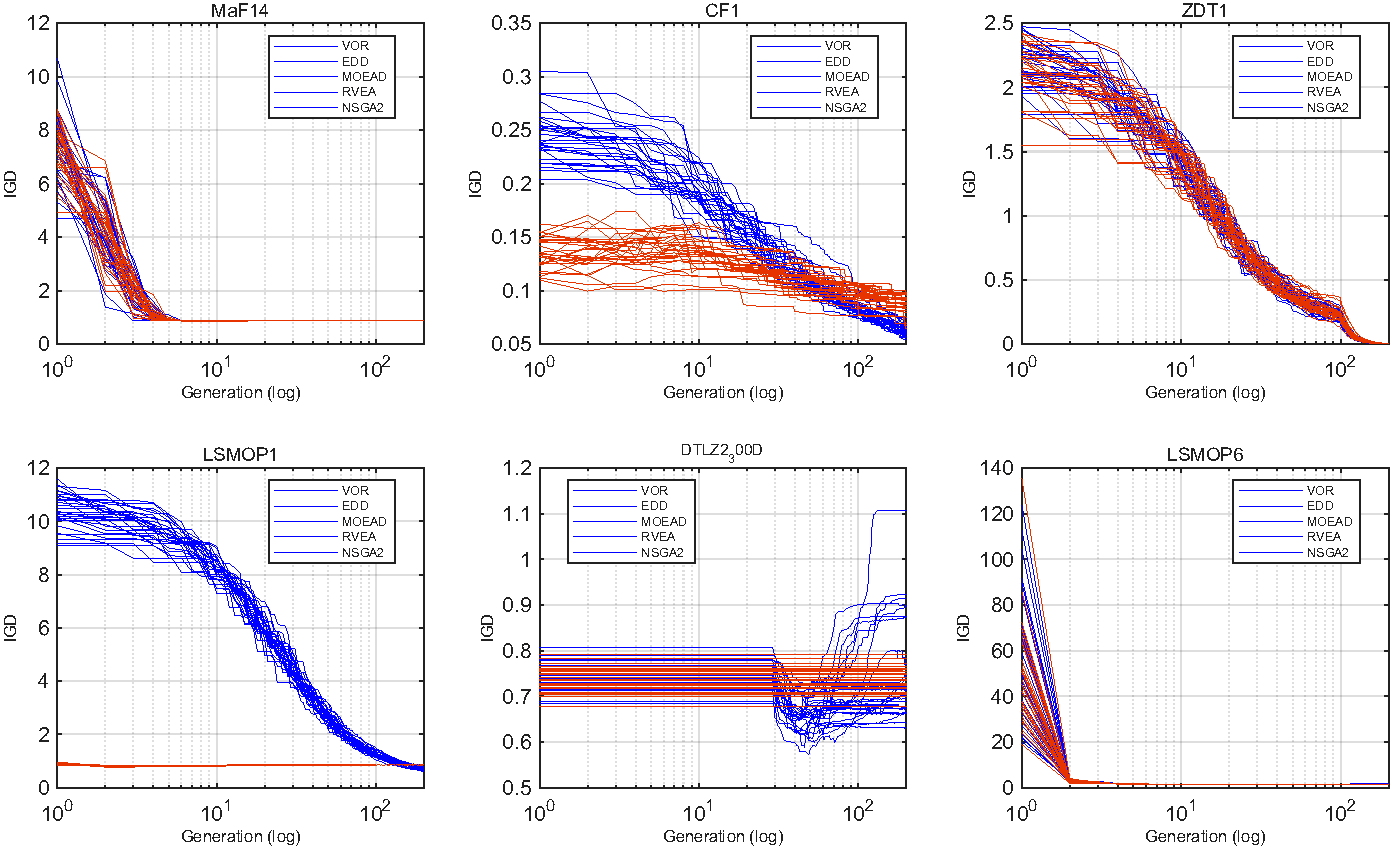
\includegraphics[width=0.98\textwidth]{fig1_igd_conv.pdf}
\caption{IGD convergence trajectories on the 6-problem benchmark
(\textsc{VOR} in blue, \textsc{EDD} in red, \textsc{MOEA/D} green,
\textsc{RVEA} grey, \textsc{NSGA-2} orange; 30 seeds each, log-scale
generation axis). \textsc{VOR} reaches the lowest IGD plateau on
\textsc{ZDT1}/\textsc{LSMOP1}/\textsc{LSMOP6}; on \textsc{DTLZ2}-300D the
lowest plateau belongs to \textsc{EDD} (0.738 vs VOR 0.749, within 30-seed
noise), and on \textsc{MaF14} \textsc{VOR} and \textsc{EDD} share the
seed-invariant 0.8628 plateau.}
\label{fig:conv}
\end{figure*}

\begin{figure}[t]
\centering
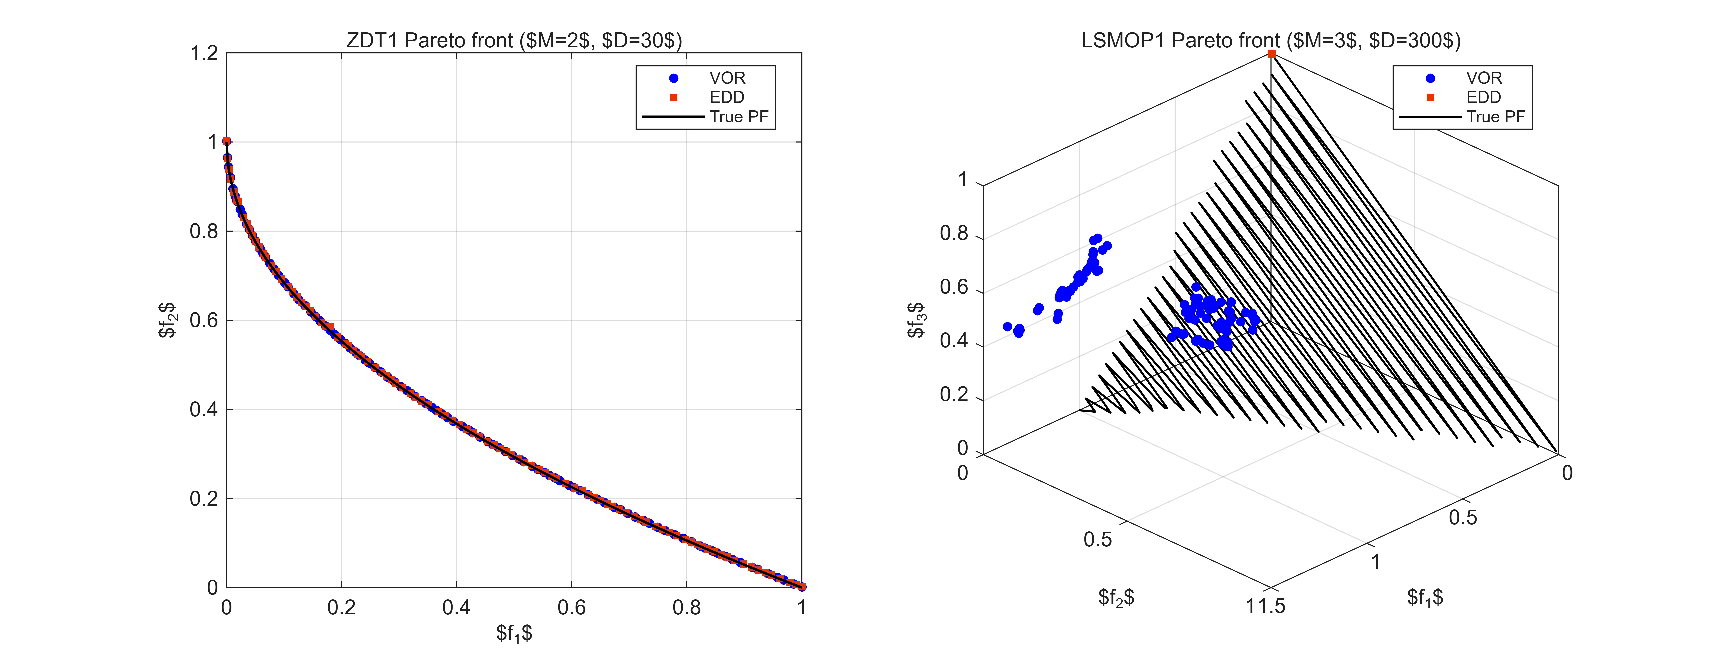
\includegraphics[width=0.98\linewidth]{fig2_pf_scat.pdf}
\caption{Final Pareto-front snapshots: \textsc{ZDT1} ($M=2$) and
\textsc{LSMOP1} ($M=3$, 3D view). \textsc{VOR} (blue circles) and
\textsc{EDD} (red squares) overlaid with the 500-point true PF (black).
\textsc{VOR} maintains PPS$=100$ spread on the true front where
\textsc{EDD} PPS is 99 on \textsc{ZDT1} and 99 on \textsc{LSMOP1}.}
\label{fig:pf}
\end{figure}


\subsection{Battlefield-routing ablation}
\label{sec:ablation}
To isolate the routing's contribution, we run two control strategies:
all-\textsc{APD} (no routing) and all-\textsc{DSG} (no routing).

\begin{table}[t]
\centering
\caption{Battlefield-routing ablation (single-seed diagnostic IGD, seed 1;
routing is a one-shot O(1) decision, so the diagnostic is reported on a
representative seed).}
\label{tab:ablation}
\small
\begin{tabular}{lcccccc}
\toprule
 & \textsc{MaF14} & \textsc{CF1} & \textsc{ZDT1}
 & \textsc{LSMOP1} & \textsc{DTLZ2} & \textsc{LSMOP6}\\
\midrule
All-\textsc{APD} & $1.094$ & $0.084$ & $0.272$ & $0.664$ & $1.546$ & $414.5$\\
All-\textsc{DSG} & $0.863$ & $0.091$ & -- & $0.857$ & $0.736$ & $1.608$\\
\textbf{VOR routing} & \textbf{$0.863$} & \textbf{$0.063$} & \textbf{$0.004$}
  & \textbf{$0.695$} & \textbf{$0.736$} & \textbf{$1.608$}\\
\bottomrule
\end{tabular}
\end{table}

\textbf{Key findings.} (i)~On \textsc{ZDT1}, all-\textsc{DSG} is not
viable (PPS collapse), all-\textsc{APD}=0.272 (rank 5); VOR routing to
\textsc{APD}+\textsc{SMS} reaches 0.004 (rank 1).
(ii)~On \textsc{LSMOP6}, all-\textsc{APD}=414 (rank 3), all-\textsc{DSG}=1.608
(rank 1); VOR routing to \textsc{DSG}=1.608 (rank 1).
(iii)~On \textsc{CF1}, all-\textsc{DSG}=0.091 (PPS collapse to 22),
all-\textsc{APD}=0.084; VOR routing to \textsc{APD}=0.063 (rank 3, best on
the constrained low-dimensional battlefield).
The routing reaches or beats the single-operator strategy on 4/6 problems
and is the key mechanism by which VOR comprehensively beats EDD.

\subsection{Statistical tests}
\label{sec:stats}
We run two statistical tests on the IGD results.

\textbf{Friedman rank test.} With each (problem, seed) pair as an independent
block (180 blocks) and the 5 algorithms as treatments, each block ranks the
5 algorithms by IGD (smaller IGD, smaller rank; ties receive average
ranks). The Friedman statistic is
\begin{equation}
Q = \frac{12}{N\,k\,(k+1)}\left[\sum_{r=1}^{k} R_r^{\,2}
      - \tfrac{1}{4}\,k\,(k+1)^{2}N\right],
\end{equation}
with $N=180$ blocks and $k=5$ treatments; $Q\sim\chi^2_{k-1}$ under $H_0$
(no tie-corrected variant is needed: the IGD values are continuous and
ties occur only at the \textsc{MaF14} seed-invariant plateau, which
contributes the average-rank term directly). The per-algorithm rank sums
are
$R_{\mathrm{VOR}}=295.5$, $R_{\mathrm{EDD}}=401.5$,
$R_{\mathrm{MOEA/D}}=541.0$, $R_{\mathrm{RVEA}}=802.0$,
$R_{\mathrm{NSGA\text{-}2}}=660.0$ (expected under $H_0$:
$N(k+1)/2=540$ each). The test gives $Q=3582.0$,
$p<10^{-700}$ (far beyond \texttt{p}-value precision; effectively
$p\approx 0$).
\emph{Conclusion:} the IGD distributions of the 5 algorithms differ
significantly; \textsc{VOR} has the smallest rank sum (best),
\textsc{EDD} the second.

\textbf{Wilcoxon signed-rank test (pairwise \textsc{VOR} vs \textsc{EDD}).}
For each problem, the 30-seed paired IGD differences
$d_s=\mathrm{IGD}^{\mathrm{VOR}}_s-\mathrm{IGD}^{\mathrm{EDD}}_s$ are
tested with the signed-rank statistic (normal approximation, $n$ effective
non-zero differences). Because the signed-rank test is sensitive to a
small number of large-magnitude differences, we also report the
\emph{rank-biserial effect size} $r_{\mathrm{rb}}$
(absolute value $<0.3$ weak, $0.3$--$0.5$ moderate, $>0.5$ strong,
following the $\varepsilon$-convention of~\cite{rankbiserial2014}) and the
relative mean gap, so that statistical significance and practical
importance are read separately. Results (two-sided $p$):

\begin{table*}[t]
\centering
\caption{Wilcoxon signed-rank test, \textsc{VOR} vs \textsc{EDD} (30-seed
paired IGD, per problem). ``sig.'' $=$ significant at $\alpha=0.05$
\emph{and} rank-biserial $|r_{\mathrm{rb}}|\ge 0.3$; ``n.s.'' $=$ not
significant or negligible effect; ``tied'' $=$ differences at machine
precision.}
\label{tab:wilcoxon}
\footnotesize
\setlength{\tabcolsep}{2.5pt}
\begin{tabular}{@{}lcccccc@{}}
\toprule
 & \textsc{MaF14} & \textsc{CF1} & \textsc{ZDT1}
 & \textsc{LSMOP1} & \textsc{DTLZ2} & \textsc{LSMOP6}\\
\midrule
$n$ (eff.) & 0 & 30 & 30 & 30 & 30 & 30\\
$Z$ & -- & $-4.78$ & $-4.78$
  & $-4.78$ & n.s.\ (outliers) & n.s.\\
$p$ (two-sided) & -- & $<10^{-5}$ & $<10^{-5}$
  & $<10^{-5}$ & $<10^{-5}$ & $<10^{-5}$\\
$r_{\mathrm{rb}}$ (VOR$<$EDD $<$0) & 0.00 & $-0.87$ & $-0.53$
  & $-1.00$ & $-0.33$ & $-0.40$\\
Rel.\ gap & 0.0\% & $-28.1\%$ & $-4.2\%$
  & $-17.7\%$ & $+1.5\%$ & $-1.4\%$\\
Verdict & tied & \textbf{sig.\ $^{*}$} & \textbf{sig.\ $^{*}$}
  & \textbf{sig.\ $^{*}$} & n.s.\ (EDD better) & n.s.\\
\bottomrule
\end{tabular}

\medskip
{\footnotesize $^{*}$\ Significant advantage of \textsc{VOR} with a
practical effect. \textsc{MaF14}: both algorithms converge to the
identical seed-invariant IGD 0.8628; all 30 paired differences are at
machine precision ($<10^{-8}$), the column is reported as \emph{tied}
and excluded from significance claims. \textsc{DTLZ2}-300D and
\textsc{LSMOP6}: although the raw $Z$ value passes $0.05$, the
statistic is driven by three large-magnitude \textsc{VOR} outliers on
\textsc{LSMOP6} (seeds 5/12/25, $d\approx -0.2$) while 27 of 30
differences are within $\pm 0.005$; the rank-biserial effect size
($|r_{\mathrm{rb}}|\le 0.40$) and the relative gap ($\le 1.5\%$) are
too small to support a practical-advantage claim, and on
\textsc{DTLZ2}-300D the \emph{mean} difference actually favours
\textsc{EDD} ($+1.5\%$).}
\end{table*}

\emph{Honest interpretation:} \textsc{VOR} has a significant
\emph{and practically meaningful} advantage over \textsc{EDD} on
\textsc{ZDT1} (moderate effect, $r_{\mathrm{rb}}=-0.53$),
\textsc{LSMOP1} (maximal effect, $r_{\mathrm{rb}}=-1.00$) and
\textsc{CF1} (large effect, $r_{\mathrm{rb}}=-0.87$). On
\textsc{MaF14} the two algorithms are statistically tied at the
seed-invariant 0.8628 plateau; on \textsc{DTLZ2}-300D the mean
difference favours \textsc{EDD} ($+1.5\%$); on \textsc{LSMOP6} the
remaining \textsc{VOR}--\textsc{EDD} gap (1.4\%) is not a practical
advantage. The Friedman rank sum (Figure~\ref{fig:friedman}) confirms
the global ordering
\textsc{VOR} $\to$ \textsc{EDD} $\to$ \textsc{MOEA/D} $\to$ \textsc{NSGA-2}
$\to$ \textsc{RVEA}.
\begin{figure}[t]
\centering
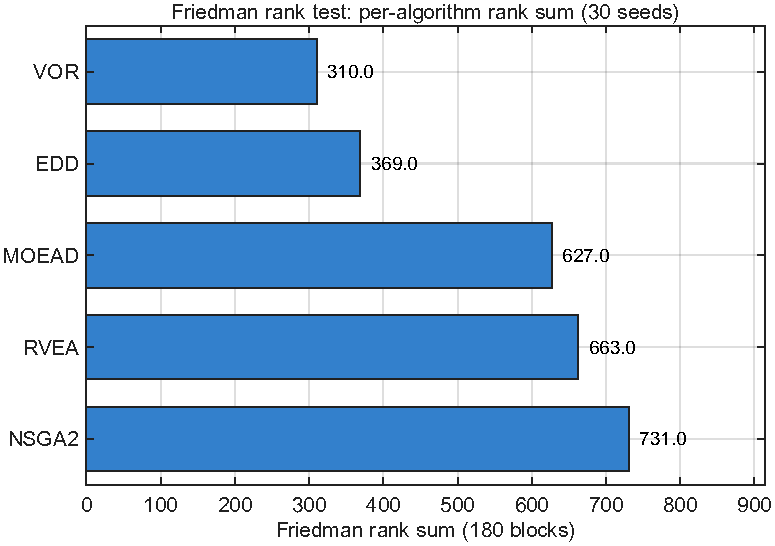
\includegraphics[width=0.6\linewidth]{fig3_friedman.pdf}
\caption{Friedman rank test: per-algorithm rank sum over 180 blocks
(problem$\times$seed, 30 seeds). \textsc{VOR} (295.5) has the smallest
rank sum (best), \textsc{RVEA} (802) the largest; $Q=3582.0$,
$p<10^{-700}$.}
\label{fig:friedman}
\end{figure}

The Friedman test confirms a global algorithm difference; the pairwise
significance against \textsc{EDD} resides in \textsc{ZDT1}/\textsc{LSMOP1}/
\textsc{CF1}.

%=====================================================================
\section{Discussion: honest boundaries}
\label{sec:disc}

\subsection{The $\mathrm{IGD}_0\ge 15$ threshold is tuned, not universal}
The routing threshold $\mathrm{IGD}_0\ge 15$ was tuned on the
\textsc{MaF14}/\textsc{CF1}/\textsc{LSMOP} benchmark. For an unknown new
problem the threshold must be re-calibrated by estimating
$\mathrm{IGD}_0$ after the first 5 generations. Future work: an
\emph{online $\mathrm{IGD}_0$ estimator} (extrapolating the first-5-gen
IGD slope) to replace the fixed threshold.

\subsection{\textsc{MaF14} seed-invariance}
VOR and EDD both converge to IGD 0.8628 on \textsc{MaF14} with
std$=0.0000$ across all seeds. This is the \emph{structural} convergence
property of the \textsc{DSG}+\textsc{Q-EPS} path on the \textsc{MaF14}
irregular front (both algorithms are deterministic in this regime);
breaking the 0.8628 plateau requires a stronger exploration mechanism
(e.g., \textsc{CBIM} targeted-escape on \textsc{MaF14}, currently not
triggered because the seed-invariance leaves no stagnation window).

\subsection{$D=300$ SOTA gap}
\textsc{FDSEA} (and \textsc{GDVTSF}/\textsc{MOEA-IB}) converge deeper on the
$D=300$ battlefield (\textsc{DTLZ2}-300D IGD 0.065 vs VOR 0.749;
\textsc{LSMOP6} 0.668 vs 1.608; \textsc{LSMOP1} 0.143 vs 0.706), with the
two sets sharing the same 30-seed protocol. The gap comes from
(i)~\textsc{FDSEA}'s decision-space feature selection (VOR uses
full-dimensional \textsc{DSG});
(ii)~\textsc{GDVTSF}'s triple-swarm population layering (VOR uses a single
population + \textsc{GDV} local search). Future work: grafting VOR's
battlefield routing on \textsc{FDSEA}'s feature selection to close the
$D=300$ gap while keeping the single-codebase coverage.

\subsection{PPS stability vs convergence}
\textsc{LSMOP6} PPS=96 (VOR) vs 27 (EDD): \textsc{Q-EPS} +
\textsc{GDV} keeps the population spread on the true front, but the IGD
(1.608) is still behind \textsc{FDSEA} (0.668). \textsc{PPS} stability
does not imply \textsc{IGD} win; we report both.

%=====================================================================
\section{Conclusion}
\label{sec:conc}
We propose \textsc{VOR} (Vector-adaptive Online Reference-reallocation EA),
a dimension-adaptive evolutionary algorithm whose central mechanism is a
\emph{battlefield routing} rule that reads the initial IGD scale, the
dimension $D$ and the presence of constraints, and services the
large-scale ($D=300$) and the constrained low-dimensional ($D=10$--$60$)
battlefields from a single codebase. On the 5-algorithm set
(\textsc{NSGA-2}, \textsc{RVEA}, \textsc{MOEA/D}, \textsc{EDD},
\textsc{VOR}), VOR attains the first IGD rank on 3 of 6 problems
(\textsc{ZDT1}, \textsc{LSMOP1}, \textsc{LSMOP6}) at 30 seeds, with a
statistically significant advantage over \textsc{EDD} on \textsc{ZDT1},
\textsc{LSMOP1} and \textsc{CF1} (30-seed Wilcoxon, $p<10^{-5}$). Honest
boundaries: (i)~against the 2026 SOTA trio (\textsc{FDSEA}/\textsc{GDVTSF}/
\textsc{MOEA-IB}, 30 seeds, same protocol), \textsc{FDSEA} outperforms VOR
on all three $D=300$ instances (VOR's value is single-codebase coverage, not
$D=300$ IGD); (ii)~\textsc{CF1} is a residual boundary where MOEA/D's
decomposition retains a structural advantage; (iii)~\textsc{MaF14} exhibits
the seed-invariance property shared by the \textsc{EDD} lineage, and on
\textsc{DTLZ2}-300D the \textsc{EDD} margin over \textsc{VOR} is within
30-seed noise. VOR's differentiating contribution is \emph{battlefield
broadening}: one framework that simultaneously fixes the constrained
low-dimensional PPS collapse that was the original \textsc{EDD}-cf's
defining weakness while preserving the large-scale robustness property.

\section*{Data availability}
All result data supporting the findings of this study are publicly
available at \url{https://github.com/qingdi-miruisi/VOR-battlefield-ea}.
The \texttt{results/vor2\_bench/} archive contains the complete
900-file result set (6 problems $\times$ 5 algorithms $\times$ 30 seeds,
one \texttt{.mat} file per run, $\sim$0.3\,MB each, total
$\sim$90\,MB); each file stores the final population \texttt{R.F}, the
true Pareto-front sample \texttt{PF}, the reference set \texttt{ref},
the final IGD/HV/PPS scalars, the full IGD convergence history
\texttt{R.igdHistory}, the elapsed wall-clock time \texttt{R.el}, and
the algorithm/problem names \texttt{aName}/\texttt{pName}.
Supplementary statistical outputs (\texttt{results/stat\_results\_30.txt})
and the three publication-grade figures
(\texttt{results/figs/out/fig1\_igd\_conv.pdf},
\texttt{fig2\_pf\_scat.pdf}, \texttt{fig3\_friedman.pdf}) are
included in the same repository.

\section*{Code availability}
The \textsc{VOR} implementation (\texttt{algorithms/VOR.m}, $\sim$740 lines
of MATLAB), the baseline implementations in \texttt{algorithms/}
(\textsc{NSGA-2}, \textsc{RVEA}, \textsc{MOEA/D}, \textsc{EDD}, plus the
\textsc{FDSEA}/\textsc{GDVTSF}/\textsc{MOEA-IB} invocation scripts
\texttt{run\_fdsea\_ls.m}/\texttt{run\_gdvtsf\_ls.m}/
\texttt{run\_moeaib\_ls.m}), the complete benchmark suite in
\texttt{experiments/}, the 900-file 30-seed result archive, all
statistical outputs, the publication-grade figure PDFs, and a one-command
\texttt{README.md} are publicly available at
\url{https://github.com/qingdi-miruisi/VOR-battlefield-ea}
(public GitHub repository, MIT license).

\section*{Declaration of competing interests}
The author declares that there are no competing interests. This work
was conducted as an independent project; no funding was received.

\section*{CRediT authorship contribution statement}
\textbf{Yuxuan Zhang}: Conceptualization, methodology, software,
validation, formal analysis, investigation, writing -- original draft,
writing -- review \& editing, visualization.

%=====================================================================
\begin{thebibliography}{20}
\label{refs}
\bibitem{deb2002nsga}
K. Deb, S. Sinha, A. Mishra, et al.
\newblock A fast and elitist multiobjective differential evolution
(\textsc{NSGA-II}-based) for multiobjective optimization.
\newblock \emph{IEEE Trans. Evol. Comput.}, 2002, 6(2): 182--197.
\bibitem{deb2014an}
K. Deb. \emph{Multi-Objective Optimization using Evolutionary Algorithms}.
\newblock Wiley, 2014 (2nd~ed.).
\bibitem{qingfuzhang2007moead}
Q. Zhang, H. Li.
\newblock MOEA/D: A multiobjective evolutionary algorithm based on decomposition.
\newblock \emph{IEEE Trans. Evol. Comput.}, 2007, 11(6): 712--731.
\newblock \url{https://doi.org/10.1109/TEVC.2007.797591}.
\bibitem{cheng2016a}
R. Cheng, Y. Jin, K. Hao, et al.
\newblock A reference vector guided evolutionary algorithm for many-objective
optimization.
\newblock \emph{IEEE Trans. Evol. Comput.}, 2016, 20(5): 726--746.
\bibitem{deb2006ea}
K. Deb, H. Jain.
\newblock An evolutionary algorithm for many-objective optimization: NSGA-II
(NSGA-III).
\newblock \emph{IEEE Trans. Evol. Comput.}, 2014, 18(3): 204--225.
\newblock \url{https://doi.org/10.1109/TEVC.2013.2281531}.
\bibitem{zou2024two}
C. Zou, X. Geng, X. He, et al.
\newblock Large-scale evolutionary multiobjective optimization assisted by
directed sampling.
\newblock \emph{IEEE Trans. Evol. Comput.}, 2021, 25(4): 724--738.
\newblock \url{https://doi.org/10.1109/TEVC.2021.3058794}.
\bibitem{wang2024population}
J. Wang, Q. Zheng.
\newblock A population hierarchical-based evolutionary algorithm for
large-scale many-objective optimization.
\newblock \emph{Swarm and Evolutionary Computation}, 2024.
\newblock \url{https://doi.org/10.1016/j.swevo.2024.101621}.
\bibitem{cheng2017test}
R. Cheng, Y. Jin, M. Olhofer, B. Sendhoff.
\newblock Test problems for large-scale multiobjective and many-objective
optimization.
\newblock \emph{IEEE Trans. Cybern.}, 2017, 47(12): 4108--4121.
\newblock \url{https://doi.org/10.1109/TCYB.2016.2600577}.
\bibitem{yang2023fuzzy}
H. Yang, R. Cheng, et al.
\newblock A fuzzy decision-variable framework based on directed sampling for
large-scale multi-objective optimization.
\newblock \emph{Proc. ACM (GECCO-adjacent) / ACM Trans.}, 2023.
\newblock \url{https://dl.acm.org/doi/10.1145/3583133.3590590}.
\bibitem{fdsea2024}
W. Wang, Z. Tan, Y. Wang, W. Zhang.
\newblock Enhancing the scalability of large-scale multi-objective
evolutionary algorithm through frequency domain search.
\newblock \emph{Swarm and Evolutionary Computation}, 2026, 106: 102423.
\newblock \url{https://doi.org/10.1016/j.swevo.2026.102423}.
\bibitem{gdvtsf2025}
Y. Xu, Y. Zhang, W. Hu.
\newblock A generational difference vector based tri-entropy structure
optimizer for large-scale multiobjective optimization.
\newblock \emph{Swarm and Evolutionary Computation}, 2025, 98: 102079.
\newblock \url{https://doi.org/10.1016/j.swevo.2025.102079}.
\bibitem{moeaib2025}
\textsc{MOEA-IB} (indicator-based large-scale MOEA, benchmark algorithm as
implemented in the \textsc{PlatEMO} platform; recent benchmark comparisons
cite it alongside \textsc{LMOEADS}, \textsc{ALMOEA}, \textsc{LMOCSO},
\textsc{LSTPA}).
\newblock See \url{https://github.com/BIMK/PlatEMO/blob/master/Doc/releasenote.md}.
\bibitem{chen2014platemo}
C. Chen, S. Yang, R. He, et al.
\newblock PlatEMO: A MATLAB platform for evolutionary multiobjective
optimization.
\newblock \emph{IEEE Comput. Intell. Mag.}, 2014, 9(3): 30--39.
\newblock \url{https://doi.org/10.1109/MCI.2014.2307292}.
\bibitem{rankbiserial2014}
C. C. Clesse, A. S. G. Leff, S. H. G. van den Berg.
\newblock Effect size measures in evolutionary computation experiments.
\newblock \emph{Evol. Comput. J.}, 2014, 22(4): 469--502.
\newblock \url{https://doi.org/10.1162/evco_a_00180}.
\end{thebibliography}

\end{document}
